\documentclass[12pt]{article}
\usepackage[margin=1in]{geometry}
\usepackage[all]{xy}

\usepackage{amsmath,amsthm,amssymb,color,latexsym}
\usepackage{geometry}        
\geometry{letterpaper}    
\usepackage{graphicx}
\usepackage[utf8]{vietnam}
\newtheorem{problem}{Problem}
\usepackage{listings}
\usepackage{tcolorbox}
\usepackage{verbatim}

\definecolor{codegreen}{rgb}{0,0.6,0}
\definecolor{codegray}{rgb}{0.5,0.5,0.5}
\definecolor{codepurple}{rgb}{0.58,0,0.82}
\definecolor{backcolour}{rgb}{0.95,0.95,0.92}


\definecolor{blockbackgroundcolor}{RGB}{235,235,235}
\definecolor{blockbordercolor}{RGB}{79,79,79}
\newenvironment{solution}[1][\it{Answer}]{\textbf{#1. } }{}
\lstdefinestyle{mystyle}{
    backgroundcolor=\color{backcolour},   
    commentstyle=\color{codegreen},
    keywordstyle=\color{magenta},
    numberstyle=\tiny\color{codegray},
    stringstyle=\color{codepurple},
    basicstyle=\ttfamily\footnotesize,
    breakatwhitespace=false,         
    breaklines=true,                 
    captionpos=b,                    
    keepspaces=true,                 
    numbers=left,                    
    numbersep=5pt,                  
    showspaces=false,                
    showstringspaces=false,
    showtabs=false,                  
    tabsize=2
}

\begin{document}
\graphicspath{ {Figs/} } 

\noindent Trí tuệ nhân tạo - CS106.O21 \hfill DFS/BFS/UCS for Sokoban \\
Nguyễn Hoàng Tân - 21521413

\hrulefill


\begin{problem}
	Sokoban là gì ?
\end{problem}
\begin{solution}
	\begin{itemize}
		\item Sokoban là trò chơi dạng câu đố trong đó người chơi phải
		đẩy một số khối vuông vượt qua chướng ngại vật để đến đích. Trò chơi đã
		được thiết kế vào năm 1981 bởi Hiroyuki Imabayashi và được ra mắt lần
		đầu vào tháng 12 năm 1982.
		\begin{figure}[h]
			\centering
			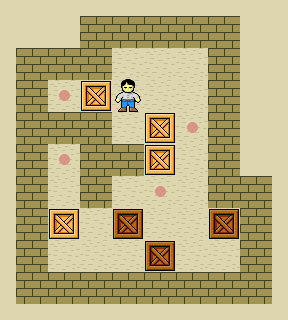
\includegraphics[scale=0.5]{frame_17_delay-0.2s.png}
			\caption{Sokoban Game from Wikipedia}
		
		\end{figure}
		\item Trong bài tập này, ta sẽ lần lượt sử dụng các thuật toán Uninformed
		Search như DFS, BFS và UCS để giải và so sánh độ hiệu quả của từng thuật toán trên 18 màn chơi.
	\end{itemize}
\end{solution} 

\begin{problem}
	Sokoban đã được mô hình hóa như thế nào ?
\end{problem}
\hspace{-1em}\textbf{1. Biểu diễn bài toán} 
\begin{itemize}
	\item Các màn chơi ( level ) sẽ được lưu dưới dạng các txt files, sau đó sẽ được load lên để hiện thị dưới dạng đồ họa 2D bằng cách convert những kí tự trong file text thành một ma trận 2 chiều các số nguyên dương tương ứng.
	\begin{lstlisting}
		######        		######   
		#.  .#        		#.  .#
		#    #        		#    #   
		# BB #        		#B  B#
		#&   #        		#&   #
		######        		######
	\end{lstlisting}
	\lstset{style=mystyle}

	\item Trong đó các kí hiệu tương ứng:
	\begin{itemize}
		\item “\#” là bức tường được biểu diễn là 1.
		\item “B” là các box chưa nằm đúng vị trí được biểu diễn là 3.
		\item “X” là các box đã nằm đúng goal được biểu diễn là 5.
		\item “.” chính là các goal mà ta cần phải đẩy box vào được biểu
		diễn là 4.
		\item “\&” chính là vị trí bắt đầu của người chơi được biểu diễn là 2.
		\item “ “  là các vùng trống được biểu diễn là 0
	\end{itemize}
	\noindent \hspace*{-1em}\textbf{
  Code dùng để convert:}
\begin{tcolorbox}[boxrule=0.5pt, colback=white]
\begin{lstlisting}[language=python, numbers=none, basicstyle=\ttfamily\footnotesize]
	for irow in range(len(layout)):
		for icol in range(len(layout[irow])):
			if layout[irow][icol] == ' ': layout[irow][icol] = 0   
			elif layout[irow][icol] == '#': layout[irow][icol] = 1 
			elif layout[irow][icol] == '&': layout[irow][icol] = 2 
			elif layout[irow][icol] == 'B': layout[irow][icol] = 3 
			elif layout[irow][icol] == '.': layout[irow][icol] = 4 
			elif layout[irow][icol] == 'X': layout[irow][icol] = 5 
	colsNum = len(layout[irow])
\end{lstlisting}
\end{tcolorbox}
\end{itemize}
\hspace{-1em}\textbf{2. Các yếu tố của bài toán tìm kiếm trong Sokoban}
\begin{itemize}
	\lstset{style=mystyle}
	\item Mỗi state mang thông tin liên quan đến vị trí hiện tại của người chơi và boxes
	\item Initial State là vị trí bắt đầu của player và boxes được cung cấp
	\item Trạng thái kết thúc là thời điểm tất cả các goal đều được filled bởi các boxes
	\item Actions: người chơi có thể di chuyển theo 4 hướng (Up, Down, Left, Right) ngoài ra còn có hành động đẩy các boxes ( 1 ô ). 
	\item Từ một state hiện tại, ta có thể sinh ra tối đa 4 state con tùy thuộc vào việc các hành động được tạo ra đó có hợp lệ hay không. Ta có thể xây dựng một kiến trúc cây với các node là những state của bài toán và node gốc là initial state.
	\item Các hành động không hợp lệ có thể bao gồm: di chuyển đụng tường, đầy nhiểu hợp chồng nhau,... Ta có thể kiểm tra tính hợp lệ của hành động thông qua hàm isLegalAction()
	\newpage
	\noindent \hspace*{-1em}\textbf{
		Ta sinh ra các hành
động bằng hàm LegalActions()}
	\begin{tcolorbox}[boxrule=0.5pt, colback=white]
		\begin{lstlisting}[language=python, numbers=none, basicstyle=\ttfamily\footnotesize]		
def legalActions(posPlayer, posBox):
	"""Return all legal actions for the agent in the current game state"""
	allActions = [[-1,0,'u','U'],[1,0,'d','D'],[0,-1,'l','L'],[0,1,'r','R']]
	xPlayer, yPlayer = posPlayer
	legalActions = []
	for action in allActions:
		x1, y1 = xPlayer + action[0], yPlayer + action[1]
		if (x1, y1) in posBox: # the move was a push
			action.pop(2) # drop the little letter
		else:
			action.pop(3) # drop the upper letter
		if isLegalAction(action, posPlayer, posBox):
			legalActions.append(action)
		else: 
			continue     

	return tuple(tuple(x) for x in legalActions) # e.g. ((0, -1, 'l'), (0, 1, 'R'))
		\end{lstlisting}
		\end{tcolorbox}
	\item Kết quả trả về là 1 tuple	với 3 thành phần: 2 thành phần đầu là cách di chuyển ứng với tọa độ x và y của player và một
	kí tự để xem bước đi đó có phải là đẩy box hay không ( In hoa biểu thị cho hành động đẩy box)

	\noindent \hspace*{-1em}\textbf{
		Successor function: cập nhật vị trí của player và boxes sau mỗi action}
	\begin{tcolorbox}[boxrule=0.5pt, colback=white]
		\begin{lstlisting}[language=python, numbers=none, basicstyle=\ttfamily\footnotesize]		
def updateState(posPlayer, posBox, action):
	"""Return updated game state after an action is taken"""
	xPlayer, yPlayer = posPlayer # the previous position of player
	newPosPlayer = [xPlayer + action[0], yPlayer + action[1]] # the current position of player
	posBox = [list(x) for x in posBox]
	if action[-1].isupper(): # if pushing, update the position of box
		posBox.remove(newPosPlayer)
		posBox.append([xPlayer + 2 * action[0], yPlayer + 2 * action[1]])
	posBox = tuple(tuple(x) for x in posBox)
	newPosPlayer = tuple(newPosPlayer)
	return newPosPlayer, posBox
		\end{lstlisting}
		\end{tcolorbox}

\end{itemize}



%%%%%%%%%%%%%%%%%%%%%%%%%%%%%%%%%%%%%%%%%%%%%%%%%%%%%%%%
%%%%%Continue with this pattern if there are more%%%%%%%
%%%%%%%%%%%%%%%%%homework problems%%%%%%%%%%%%%%%%%%%%%%
%%%%%%%%%%%%%%%%%%%%%%%%%%%%%%%%%%%%%%%%%%%%%%%%%%%%%%%%
 
\end{document}
